\documentclass{standalone}
\usepackage{tikz}
\usepackage{ctex,siunitx}
\usepackage{tkz-euclide}
\usepackage{amsmath}
\usetikzlibrary{patterns, calc}
\usetikzlibrary {decorations.pathmorphing, decorations.pathreplacing, decorations.shapes,}
\begin{document}
\small
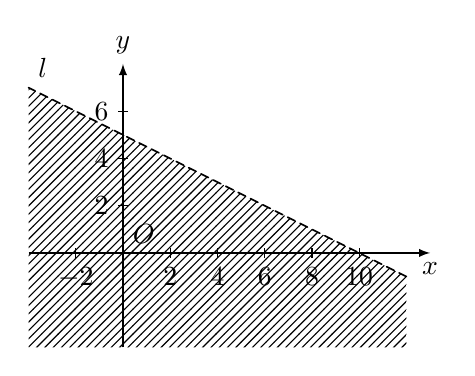
\begin{tikzpicture}[>=latex,scale=0.3]
  \draw[thin,->](-4,0)--(13,0)node[below]{$x$};
  \draw[thin,->](0,-4)--(0,8)node[above]{$y$};
  \tkzDefPoints{0/0/O,-4/7/M,12/-1/N,-4/-4/P,12/-4/Q}
  \foreach \x in {-2,2,4,6,8,10}
  {
    \draw[thin](\x,-0.2)--++(0,0.4)node[at start,below]{$\x$};
  }
  \foreach \x in {2,4,6}
  {
    \draw[thin](0.2,\x)--++(-0.4,0)node [left]{$\x$};
  }
  \tkzDrawLine[semithick,densely dashed,add= 0 and 0](N,M)
  \tkzLabelLine[pos= 1.0,above right](N,M){$l$}
  \fill[pattern=north east lines](N)--(M)--(P)--(Q);
  \tkzLabelPoints[above right](O)
\end{tikzpicture}
\end{document}